% mn2esample.tex
%
% v2.1 released 22nd May 2002 (G. Hutton)
%
% The mnsample.tex file has been amended to highlight
% the proper use of LaTeX2e code with the class file
% and using natbib cross-referencing. These changes
% do not reflect the original paper by A. V. Raveendran.
%
% Previous versions of this sample document were
% compatible with the LaTeX 2.09 style file mn.sty
% v1.2 released 5th September 1994 (M. Reed)
% v1.1 released 18th July 1994
% v1.0 released 28th January 1994

\documentclass[useAMS,usenatbib]{mn2e}
\usepackage{graphicx}
\usepackage{amsmath}


% If your system does not have the AMS fonts version 2.0 installed, then
% remove the useAMS option.
%
% useAMS allows you to obtain upright Greek characters.
% e.g. \umu, \upi etc.  See the section on "Upright Greek characters" in
% this guide for further information.
%
% If you are using AMS 2.0 fonts, bold math letters/symbols are available
% at a larger range of sizes for NFSS release 1 and 2 (using \boldmath or
% preferably \bmath).
%
% The usenatbib command allows the use of Patrick Daly's natbib.sty for
% cross-referencing.
%
% If you wish to typeset the paper in Times font (if you do not have the
% PostScript Type 1 Computer Modern fonts you will need to do this to get
% smoother fonts in a PDF file) then uncomment the next line
% \usepackage{Times}

%%%%% AUTHORS - PLACE YOUR OWN MACROS HERE %%%%%

\title[Results of two stellar occultations by Ceres]{Results of two stellar occultations by dwarf planet (1) Ceres}
\author[A. V. Raveendran and A. N. Other]{A. V. Raveendran$^{1}$\thanks{E-mail:
email@address (AVR); otheremail@otheraddress (ANO)} and A. N.
Other$^{2}$\footnotemark[1]\thanks{This file has been amended to
highlight the proper use of \LaTeXe\ code with the class file.
These changes are for illustrative purposes and do not reflect the
original paper by A. V. Raveendran.}\\
$^{1}$Indian Institute of Astrophysics, Bangalore 560034, India\\
$^{2}$Building, Institute, Street Address, City, Code, Country}
\begin{document}

\date{Accepted 1988 December 15. Received 1988 December 14; in original form 1988 October 11}

\pagerange{\pageref{firstpage}--\pageref{lastpage}} \pubyear{2002}

\maketitle

\label{firstpage}

\begin{abstract}
Abstract
\end{abstract}

\begin{keywords}
keywords.
\end{keywords}

\section{Introduction}

Ceres is the sole exemplar of a dwarf planet in the inner Solar System. Far from being a mere taxonomic information, this suggests the great impact its study can have on the understanding of planetary formation and evolution of the Solar System. Indeed, it was proposed that Ceres could have its origin as a transneptunian object, latter scattered to the Main Belt due to the giant planets' migration predicted by the ``Nice Model''. It may well had been formed close to its current location, however, even on this scenario, the dynamical history of the Solar System must have let its signatures on Ceres. Not only on the late heavy bombardment features that might exist on its surface, but also on its volatiles, which could have been transported from the outer region.

Since the 1970's it has been speculated that Ceres could contain water ice, what was recently verified \citep{Kuppers2014}. Although the water regime on this object is still unknown, some internal structure models suggest the existence of a water ice -- or even a liquid water -- layer. Yet the very question of whether Ceres suffered differentiation is open and, on the assumption of an affirmative answer, it is natural to ask if it ever had tectonics, how its geological evolution was, and if it is still active. Inarguably, \textit{NASA}'s \textit{Dawn} mission will shed light on several open issues concerning Ceres.

Owning approximately one fifth of the whole Main Belt's mass, Ceres is expected to have an equilibrium figure, \textit{i.e.}, a Maclaurin or a Jacobi ellipsoid. In fact, direct observations of Ceres by means of adaptive optics confirmed it to be an oblate spheroid \citep{Drummond2014}. The precise knowledge of its shape and dimensions is important, for the models of density, internal structure and differentiation can depend on the size and oblateness of the body.

The best ground-based technique for determining shape and size of a faraway object is the study of its shadow, cast by a star during an occultation. Since the 1960's occultations have provided measurements of hundreds of asteroids, thanks partially to the proficuous professional-amateur collaboration on the field. More recently, this technique has been applied to objects of the outer Solar System and has unveiled outstanding features of distant bodies, \textit{e.g.}, the ring system around the Centaur (10199) Chariklo \citep{BragaRibas2014}.

The first stellar occultation by Ceres was observed in 1984 \citep{Millis1987} and lead to the determination of its size to the precision of the kilometre, at a time when the uncertainties were often ten times larger. The low apparent magnitude of Ceres, if compared to most asteroids, imposes a somewhat strong constraint on the stars capable of causing a detectable magnitude drop when occulted. For instance, after the 1984 event, to our knowledge, only four like this have been observed. Two of them had only two chords each, not sufficient, thus, for providing accurate measurements\footnote{These events took place on 22 August 1994 and 30 October 2010.}. The two remaining events, which occurred on 17 August 2010 and 25 October 2013, are reported on the present work. The former was observed in Brazil from 5 stations, while the later was from the United States and led to 9 chords. Throughout the paper we shall refer to these events as the ``2010'' and the ``2013 occultation''.

This work is organized as follows. In Sections 2 and 3 we analyse, on this order, the 2010 and the 2013 events. The comparison of both results to those on the literature is carried out in Section 4. We summarise our conclusions in Section 5.








\section[]{The 2010 occultation}

\begin{equation}
\left\{ 
  \begin{array}{l l}
    \alpha = 17^{h}18^{m}29^{s}.0080\\
    \delta = -27\degr 26\arcmin 38\arcsec.890
  \end{array}
\right.
\end{equation}

\begin{figure}
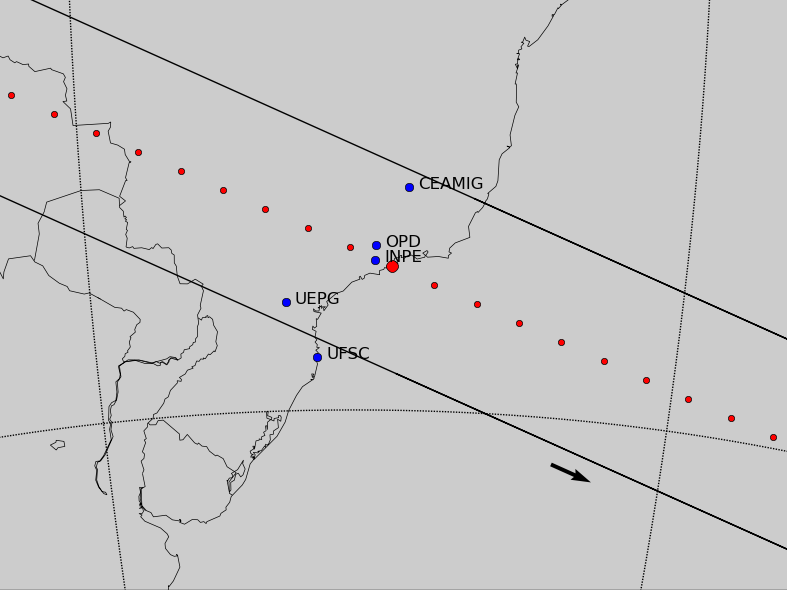
\includegraphics[scale=0.42]{figures/Ceres_2010.png} 
\caption{Post-occultation reconstruction of Ceres' shadow path on Earth for the 2010 August 17 event. The big red dot is the geocentric closest approach at 22:41:28 UT. The small red ones represents the center of the shadow separated by one minute where the shadow moves from the left to the right. The blue dots are the sites that have observed the event. As described in text, UFSC had a negative chord.
\label{Fig: Ceres-2010-map}}
\end{figure}



\subsection{Observations}

Observations were carried out in Brazil at five stations as displayed in Table 1. The occultation was detected on four of them. Among these, one started the shots with the event already in progress and only provided star's reappearance time; the other three recorded the whole phenomenon.  Since this event had a very low velocity -- only 3.9 km/s -- the exposure times (which for faster occultations would result in a big time uncertainty) led to quite small error bars, with the exception of the UEPG chord. Moreover, as the larger timing errors occurred closer to the edges of the shadow's path, their radial-projected uncertainty came to be still smaller.

[Falar sobre a quest\~ao do tempo em cada corda. A leitura do header era no segundo inteiro? Foi analisada a cad\^encia das imagens? Qual a precis\~ao?]

[Durante o per\'iodo de observac\~ao Ceres rodou apenas 3.1$\degr$. Mas isso n\~ao \'e relevante no caso de Maclaurin...]

\begin{table*}
 \centering
 \begin{minipage}{140mm}
  \caption{Circumstances of observation for all observing stations of the 2010 event.}
  \begin{tabular}{@{}lccccc}
  \hline
     Site & Longitude & Telescope & Exposure & Result & Observer  \\
          & Latitude  & Aperture  & Readout overhead  & Ingress & \\          
          & Height    & Camera    &    S/N    & Egress    & \\          
\hline
 Belo Horizonte & 43$\degr$59'51.1'' W & LX200 & 5 s & Positive & C. Jacques  \\
 CEAMIG-REA &19$\degr$49'49.0'' S & 31 cm &     & 22:39:03.9 $\pm$ 0.6 &  E. Pimentel \\
            & 825 m                &       &     & 22:40:20 $\pm$ 5 &   \\
 & & & & & \\
 Pico dos Dias    & 45$\degr$34'45.1'' W &       & 1 s & Positive & J. I. B. Camargo \\
 OPD/LNA    &22$\degr$32'03.7'' S & 60 cm &     & 22:37:30.3 $\pm$ 0.6 &  G. B. Rossi \\
            & 1864 m               &       &     & 22:41:55.3 $\pm$ 0.7 &              \\
 & & & & & \\
 S\~ao Jos\'e dos       & 45$\degr$51'44.0'' W &  C11  & 2 s & Egress only & A. C. Milone\\
 Campos       &23$\degr$12'33.0'' S & 28 cm &     & Start: 22:39:44 & T. Maldonado\\
 INPE      & 975 m                & SBIG ST7 &     & 22:42:03.0 $\pm$ 0.2 & M. Okada    \\
 & & & & & \\
 Ponta Grossa       & 50$\degr$05'56.0'' W & RCX 400 &30 s & Positive & M. Emilio   \\
 UEPG       &25$\degr$05'22.2'' S & 40 cm &     & 22:37:17 $\pm$ 13 & L. Mehret   \\
            & 910 m                & SBIG STL6E &     & 22:39:56 $\pm$ 13 & \\
 & & & & & \\
 Florian\'opolis       & 48$\degr$31'20.5'' W &       & 3 s & No occultation  & W. Schoenell\\
 UFSC       &27$\degr$36'12.3'' S & 28 cm &     &  & A. J. T. Mello\\
            & 20 m                 &       &     &         & F. R. Herpich \\
\hline
\end{tabular}
\end{minipage}
\end{table*}










\subsection{Light curves and timing}

[Curvas de luz, modelagem, difraç\~ao, di\^ametro estelar.]


\begin{figure}
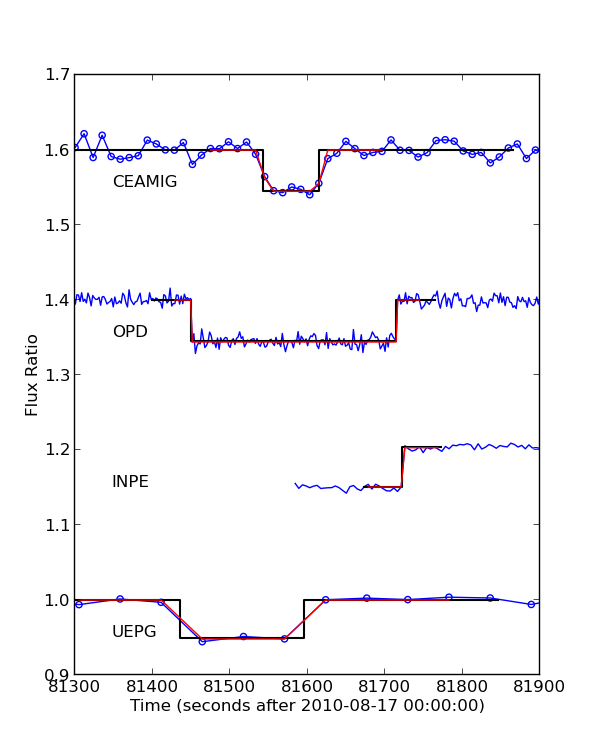
\includegraphics[scale=0.58]{figures/Ceres_2010_fluxratio.png} 
\caption{The four occultation light curves normalized and vertically shifted by a factor of 0.2 for better viewing. The solid black lines are the best fit of the square-well model to the data. The red lines are the square-well model convoluted with the Fresnel diffraction, the star diameter, and the applied exposure time. The mid-times of the occultations do not coincide due to the propagation delays of the shadow due to the distinct longitude of the sites. The exposures at INPE were started after the immersion, as explained in the text. \label{Fig: Ceres-2010-curves}}
\end{figure}


\subsection{Limb fitting methodology}

The methodology used to analyse Ceres' profile from the observations is the standard one, applied, for example, by \cite{Ortiz2012} and \cite{BragaRibas2013}. To each combination of site position and recorded ingress/egress time, together with star coordinates and Ceres' ephemeris, corresponds a point $(f_{i,obs},g_{i,obs})$ on the plane of the sky. The collection of those points ideally determines the apparent limb of Ceres.

We adopt an elliptic model for the limb profile, resulting from the projection of an oblate spheroid onto the sky plane. This model is supported by the work of \cite{Drummond2014}, by means of direct imaging of Ceres. Hence, we have $N=7$ chord extremities to adjust the $M=5$ parameters which define an ellipse: apparent semimajor and semiminor axis -- $a^\prime$ and $b^\prime$, respectively --, position angle $P$ and the position $(f_c,g_c)$ of its centre with respect to the occulted star. The first two parameters can be interchanged with the oblateness and the equivalent radius, defined, on this order, by $\epsilon^\prime = 1 - (b^\prime/a^\prime)$ and $R_{equiv} \equiv \sqrt{a^\prime b^\prime} = a^\prime\sqrt{1-\epsilon^\prime}$. We define the number of degrees of freedom of the problem as $\mathcal{N} \equiv N - M$.

Correspondence between true and apparent figures depends on the polar aspect angle $\zeta$, encompassed by the (true) polar $b$-axis and the line of sight. The apparent oblateness is related to the true one, $\epsilon$, through
%
\begin{equation}
\epsilon^\prime = 1 - \sqrt{\cos^2(\zeta) + (1-\epsilon)^2\sin^2(\zeta)}.
\end{equation}

Of course, the apparent semimajor axis $a^\prime$ equals the equatorial radius $a$ of the ellipsoid. %The polar radius $b$ can then be determined from $\epsilon = 1 - (b/a)$.

The search for the best fit ellipse is carried out by minimizing the reduced $\chi^2$ function:
%
\begin{equation}
\chi^2_r = \frac{1}{\mathcal{N}} \sum_{i=1}^N \frac{1}{\sigma_i^2}  \left[ (f_{i,obs}-f_{i,cal})^2 + (g_{i,obs}-g_{i,cal})^2\right].
\end{equation}
%
Here $\sigma_i$ is the radial uncertainty of the $i$th chord extremity, obtained by multiplying the time uncertainty reported in Table~1 by the normal velocity of the star (with respect to the limb model). $f_{i,cal}$ and $g_{i,cal}$ are the coordinates of the point on the model ellipse, where a line that goes from the centre of the model to the data point $(f_{i,obs},g_{i,obs})$ intersects the ellipse.%:
%
%\begin{equation}
%f_{i,cal} \equiv f_{i,obs} + \rho \cos(\theta), \quad g_{i,cal} \equiv %g_{i,obs} + \rho \sin(\theta),
%\end{equation}
%
%with:
%\begin{equation}
%\theta \equiv \arctan\left( \frac{g_{i,obs}-g_{c}}{f_{i,obs}-f_{c}} %\right) ,
%\end{equation}
%
%\begin{equation}
%\rho \equiv a^\prime b^\prime / \sqrt{[a^\prime\sin(\theta+P)]^2 +[b^\prime\cos(\theta+P)]^2 }.
%\end{equation}

Evaluation of the reduced $\chi^2$ function over the $\lbrace a, \epsilon^\prime, P, f_c, g_c \rbrace$--space produces a map related to the likelihood of a solution. For instance, the 1--sigma reported time uncertainties correspond to the subset of the parameter space for which $\chi^2_r$ lies between ${\chi^2_r}_{min}$ and ${\chi^2_r}_{min} + 1$. This allows the determination of the error bars of the physical parameters. It is worthwhile to mention that we consider all the uncertainty as due to timing issues.





\subsection{Limb fitting solutions}

We considered two possible solutions for the limb fitting. The first is the nominal one, which is the determination the five parameters which characterize an ellipse from the seven observed contacts. As we shortly show, it led to a rather large error bar on the position angle. Furthermore, the nominal solution solely is not capable of returning the true oblateness, which can be evaluated through equation (1), provided that the angle $\zeta$ is known.% or constrained by some physical hypothesis.

From observations by adaptive optics spanning a 9-year period, \cite{Drummond2014} determined the position of Ceres' polar axis within a range of only 3$\degr$:
\begin{equation}
%\left\{ 
%\begin{array}{l}
\alpha = (287 \pm 3) \degr, \quad %\\
\delta = (+64 \pm 3) \degr,
%\end{array} \right .
\end{equation}
%
in equatorial ICRF/J2000 coordinates. Together with Ceres' ephemeris at the moment of the occultation, this corresponds to a polar aspect angle $\zeta = 93.9\degr$, which is very close to an equator-on geometry. Hence, we expect true figures to be close to apparent ones.

The knowledge of Ceres' pole not only allows the determination of its polar aspect, it suffices to set its position angle. Therefore, (3) may act as a constraint for $P$, and a second solution can be obtained by probing the parameter space with the restriction that the position angle is confined to the range that follows from (3). We call this the ``pole-constrained solution''.


\subsubsection{Nominal solution}

With the seven observed contacts it is possible to adjust the five parameters which define an ellipse. For the best fit solution we find $\chi^2_{r,min} = 0.24$, which could be interpreted as a slightly overestimation of the error bars with regard to the good quality of the fit. However, inasmuch as the problem has only two degrees of freedom, it is far from the statistical realm and low $\chi^2_{r,min}$ may eventually happen.

The resulting values of semimajor axis, oblateness, position angle and centre coordinates are presented in the second column of Table~2.%, and the corresponding ellipse is plotted with the observed chords in Fig.~2.
% The equivalent radius of the best fit solution is $R_{equiv} = 469 \pm 10$ km.

Already mentioned, the parameter with the largest uncertainty is the position angle: spanning on a 20$\degr$ interval, its determination has a relative precision worse than 10$\%$. Clearly, the coordinates of Ceres' pole (3) can impose a strong constraint on the position angle, as the next solution shows.

Finally, the correction to the oblateness due to Ceres' polar aspect angle lies within the 1-sigma error bar and has no statistical relevance; hence $\epsilon = 0.08 \pm 0.03$.





\subsubsection{Pole-constrained solution}

At the moment of the occultation, the coordinates (3) of Ceres' rotational pole correspond to the position angle $P = (12 \pm 3)\degr$. Exploration of the parameter space, restricted to ellipses whose position angle lie on this range, results in the pole-constrained solution. The related physical parameters are displayed on the third column of Table~2.

We notice that the constraint corresponds to the upper limit of nominal solution's 1-sigma error bar. On the other hand, it selects the smallest values of semimajor axis, improving its determination by a factor of about 2. Notwithstanding, oblateness' figures remain the same.

\begin{table*}
 \centering
 \begin{minipage}{140mm}
  \caption{Results of limb fitting to the data of the 2010 and 2013 events.}
  \begin{tabular}{@{}lcccc}
  \hline
     Solution & 2010/Nominal & 2010/Pole-constrained & 2013/Nominal & 2013/Pole-constrained \\
\hline
Equatorial Radius (km) & 491 $\pm$ 7   & 486 $\pm$ 3   & 486 $\pm$ 2   & \\
Oblateness          & 0.08$\pm$0.03 & 0.08$\pm$0.03 & 0.09$\pm$0.05 & \\
Position angle (deg)& 5 $\pm$ 10    & 12 $\pm$ 3 (*)& 22 $\pm$ 5    &  \\
$f_c$ (km)          & 133 $\pm$ 9   & 138 $\pm$ 5   & 78 $\pm$ 7    & \\
$g_c$ (km)          & -17 $\pm$ 15  & -11 $\pm$ 11  & 14 $\pm$ 16   & \\
$\chi^2_{r,min}$    & 0.24          &  0.42         & 1.27          & \\
\hline
\end{tabular}
\textbf{Notes.} Error bars are at 1-sigma level. The reported oblateness derived from the 2010 event are the true ones, see text for details. \\
(*) Position angle derived from Ceres' rotational pole coordinates determined by \cite{Drummond2014}.
\end{minipage}
\end{table*}

\begin{figure}
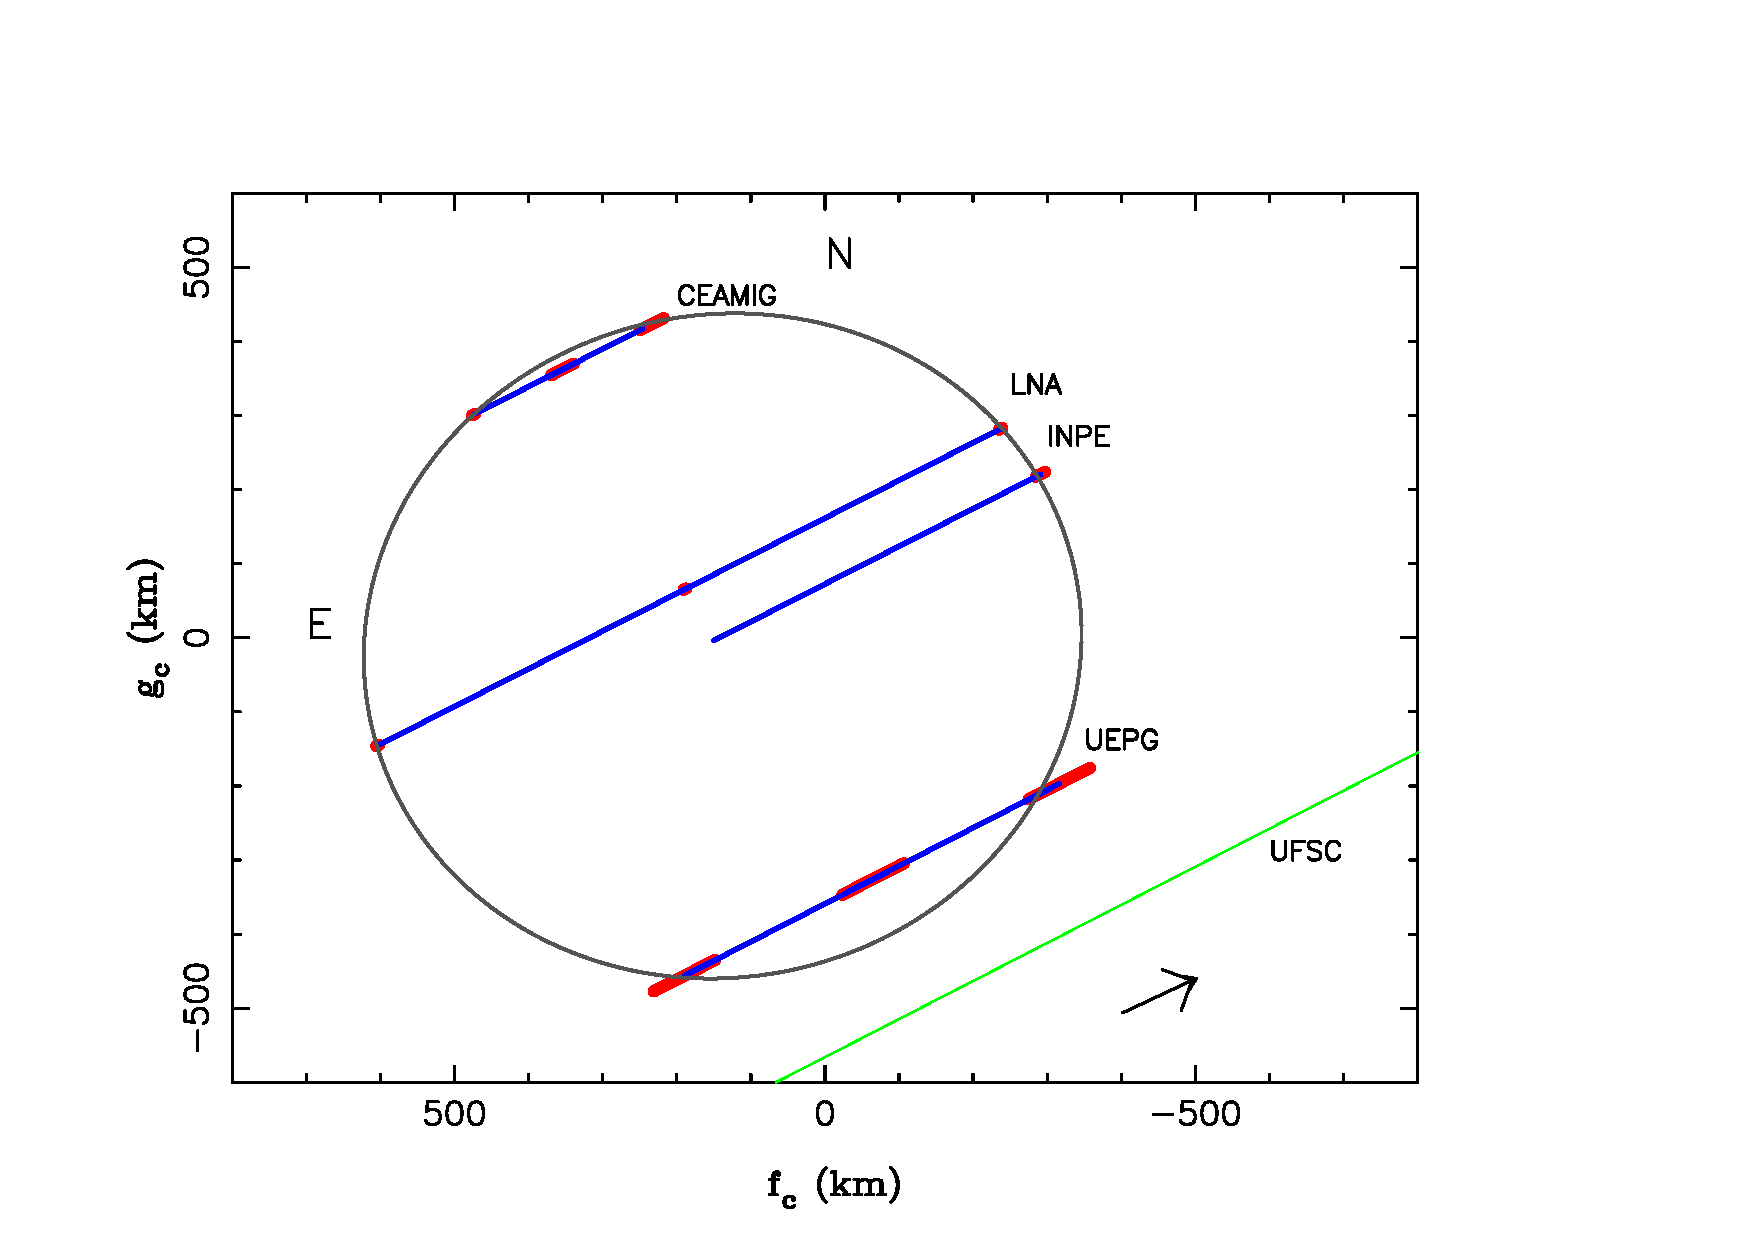
\includegraphics[scale=0.36]{figures/Ceres_2010_body.pdf} 
\caption{\label{Fig:Ceres-2010-body}}
\end{figure}

\section[]{The 2013 occultation}

\begin{equation}
\left\{ 
  \begin{array}{l l}
    \alpha = 11^{h}57^{m}52^{s}.7641\\
    \delta = +09\degr 07\arcmin 49\arcsec.835
  \end{array}
\right.
\end{equation}

\begin{figure}
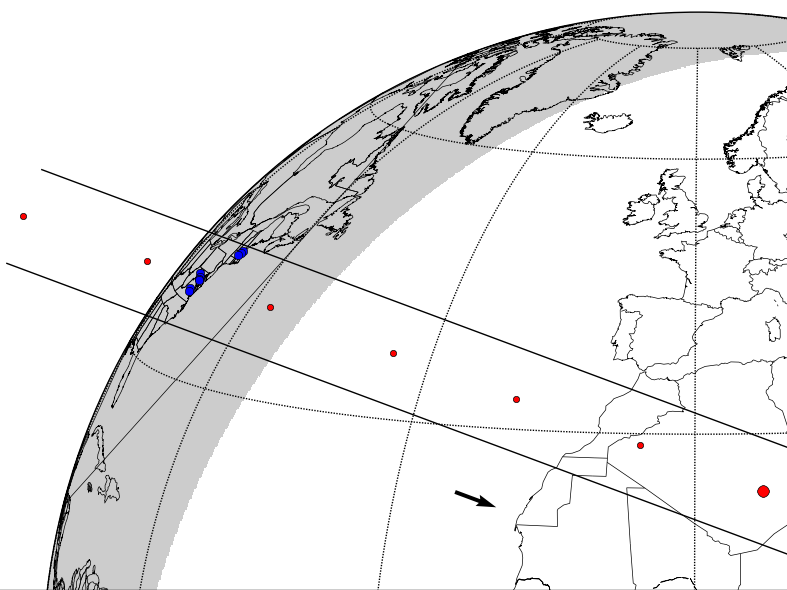
\includegraphics[scale=0.42]{figures/Ceres_2013.png} 
\caption{Post-occultation reconstruction of Ceres' shadow path on Earth for the 2013 October 25 event at the east coast of USA. The red dots represents the center of the shadow separated by one minute where the shadow moves from the left to the right. The geocentric closest approach at 09:43:11 UT. The blue dots are the sites that have observed the event.\label{Fig: Ceres-2013-map}}
\end{figure}

\subsection{Observations}\label{Sec: observation-2013}

Nine positive chords were obtained for the 2013 occutation by a variety of equipment as listed in Table \ref{Tab: obs-2013}. Each station was equipped with a video camera (whose readout time may be considered negligible). This is of particular importance in this event, since Ceres' shadow had the much faster speed of 42.6 $km/s$, if compared to the 2010 event. All the observing sites are in the United States, as depicted in Figure \ref{Fig: Ceres-2013-map}.

Three different timing synchronization procedures were adopted among the set of observing stations. At Greenbelt and Owings the 1PPS signal of a GPS unit was used to calibrate time stamps which were inserted at each frame of the video. Time extraction is thus straightforward, after taking camera delays into account. On the other hand, at Brookline the clock would be synchronized by an internet server. A lack of connection, however, resulted in spurious times. In fact, comparison between the times obtained at this station and the others suggests that the former have a delay of about 64 s. Therefore, for Brookline we do not use its absolute times in the analysis that follows. Finally, at the six stations left the videos were recorded by camcorders on digital tapes. The timing method consisted in the comparison of the camcorder internal clock to a 1PPS GPS signal, before and after the recording of the occultation. Absolute timing errors of this procedure are expected to be inferior to 0.1 s.

A remarkable observing circumstance of this event is the low altitude of Ceres with respect to the horizon. Precisely, its altitude at moment of the occultation ranged between $20\degr$ (Hampton) and $15\degr$ (Winchester). Strong scintillation is expected in such a scenario which, combined to the low magnitude drop of the event, resulted in a larger uncertainty in the time of the contacts, as it is shown in the next section.


\begin{table*}
 \centering
 \begin{minipage}{140mm}
  \caption{Circumstances of observation for the observing stations of the 2013 event.\label{Tab: obs-2013}}
  \begin{tabular}{@{}lccccc}
  \hline
     Site & Longitude & Telescope: & Camera  & Result & Observer  \\
          & Latitude  & Aperture  & Cycle time & Ingress & \\          
          & Height    & f-ratio    &    S/N    & Egress    & \\          
\hline
 Hampton & 70$\degr$48'59.7'' W & 12 cm & PC164C-EX2 & Positive & T. Blank \\
  &42$\degr$53'52.8'' N & f/5 & 0.033 s     & 09:40:46.9 $\pm$ 0.1 &   \\
            & 7 m       &  &     & 09:40:57.26  $\pm$ 0.08 &   \\
 & & & & & \\
 Topsfield & 70$\degr$55'16.6'' W & 12 cm & PC164C-EX2 & Positive & T. Blank \\
  &42$\degr$37'55.9'' N & f/5      & 0.033 s   & 09:40:45.4 $\pm$ 0.1 &   \\
            & 45 m      &  &     & 09:40:58.0  $\pm$ 0.1 &   \\
 & & & & & \\
 Brookline & 71$\degr$08'14.5'' W & 64 cm & Infinity2-1R & Positive & N. Weber \\
  &42$\degr$18'27.4'' N & f/9.6 & 0.015 s     & Duration only &  R. Dantowitz  \\
            & 109 m     &       &     & (14.93 $\pm$ 0.01) s &   \\
 & & & & & \\
 Winchester & 78$\degr$14'39.6'' W & 36 cm & PC164C & Positive & J. Brooks \\
  &39$\degr$16'21.5'' N & f/5 & 0.033 s    & 09:40:33.26 $\pm$ 0.08 &   \\
            & 211 m     &  &     & 09:40:55.86  $\pm$ 0.09 &   \\
 & & & & & \\
 Greenbelt & 76$\degr$52'09.4'' W & 12 cm & PC164C-EX2 & Positive & J. Dunham \\
  &38$\degr$59'12.1'' N & f/2.5 & 0.033 s    & 09:40:33.6 $\pm$ 0.1 & D. Dunham  \\
            & 52 m      &   &     & 09:40:56.4  $\pm$ 0.1 &   \\
 & & & & & \\
 Alexandria & 77$\degr$02'28.3'' W & 7 cm & Watec120N & Positive & P. Maley \\
  &38$\degr$49'19.1'' N & f/10 &  0.067 s   & 09:40:33.3 $\pm$ 0.1 &   \\
            & 8 m       &   &     & 09:40:56.1  $\pm$ 0.1 &   \\
 & & & & & \\
 Owings & 76$\degr$38'06.3'' W & 25 cm & PC164C  & Positive & C. Ellington \\
  &38$\degr$41'26.5'' N & f/3.3 &  0.033 s & 09:40:34.27 $\pm$ 0.05 &   \\
            & 38 m                &       &     & 09:40:56.0  $\pm$ 0.2 &   \\
 & & & & & \\
 Mechanicsville & 77$\degr$23'06.7'' W & 12 cm & PC164C-EX2 & Positive & D. Dunham \\
  &37$\degr$41'26.1'' N & f/2.5 & 0.033 s    & 09:40:33.0 $\pm$ 0.1 &   \\
            & 60 m      &   &     & 09:40:54.8  $\pm$ 0.1 &   \\
 & & & & & \\
 Varina & 77$\degr$19'49.3'' W & 12 cm & PC164C-EX2 & Positive & D. Dunham \\
  &37$\degr$25'58.6'' N & f/2.5 &  0.033 s   & 09:40:32.4 $\pm$ 0.3 &   \\
            & 19 m      &   &     & 09:40:53.1  $\pm$ 0.2 &   \\

\hline
\end{tabular}
\end{minipage}
\end{table*}

\subsection{Light curves and timing}

All videos were converted to FITS images and the flux of the star was obtained with the Platform for Reduction of Astronomical Images Automatically (PRAIA) \citep{2011gfun.conf...85A}. The light curves were normalized to an unocculted star flux when a star was available.

The data were binned by 5 or 10 points to reduce the noise. A linear or second-degree polynomial fit was applied to the observed flux before and after the occultation.

For the observations at Owings and Greenbelt, the time was inserted on each frame. For Brookline, the time was extracted from the image header. For the others, the time was obtained from the reports of IOTA. The cycle time of the images is shown in Table \ref{Tab: obs-2013}.

The start and end times of the occultation were obtained for each light curve by fitting a sharp edge occultation model. This model is convolved by Fresnel diffraction, the CCD bandwidth, the stellar diameter in kilometers, and the finite integration time; see \cite{Widemann2009}.

The Fresnel scale ($F = \sqrt{\lambda D/2}$) for the present Ceres’ geocentric distance $D = 3.28 AU = 4.91 \times 10^{8} km$ is 0.4 km for a typical wavelength of $\lambda = 0.65 \micron m$.The star diameter is estimated using the formulae of \cite{vanBelle1999}. Its B, V , and K apparent magnitudes are 10.47, 9.97 and 8.76, respectively, in the Tycho catalog \citep{Hog2000}. This yields a diameter of about 0.16 km projected at Ceres’s distance. The smallest integration time used in the positive observations was 0.033 s, which translates to almost 1.4 km in the celestial plane. Therefore, the occultation light curves are largely dominated by the integration times, not by Fresnel diffraction or star diameter.

The occultation fits consist in minimizing a classical $\chi^{2}$ function for each light curve, as described in \cite{Sicardy2011}. The free parameter to adjust is the ingress (disappearance) or egress (re-appearance) time $t_{occ}$, which provides the minimum value of $\chi^{2}$, denoted as $\chi^{2}_{min}$.

The best fits to the occultation light curves are shown in Figure \ref{Fig: Ceres-2013-curves}, and the derived occultation times are listed in Table \ref{Tab: obs-2013}.

\begin{figure}
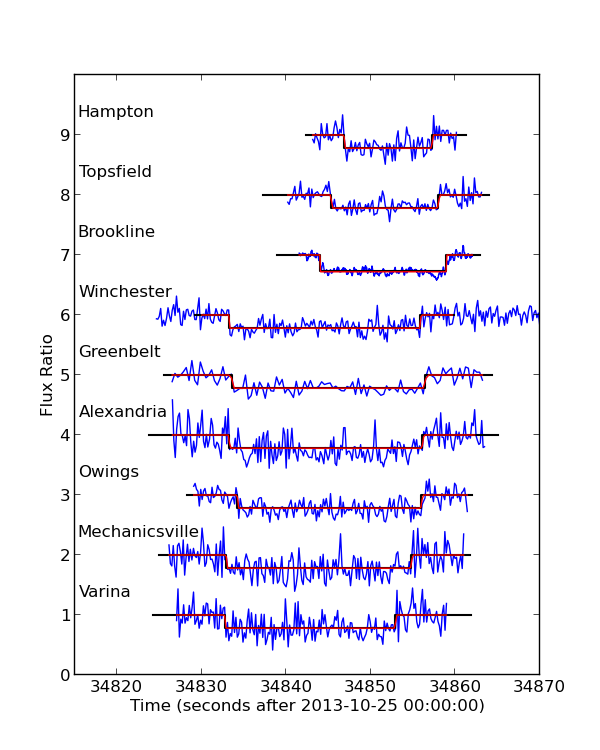
\includegraphics[scale=0.58]{figures/Ceres_2013_fluxratio} 
\caption{Same as in Fig. \ref{Fig: Ceres-2010-curves} for the nini light curves of the 2013 event. \label{Fig: Ceres-2013-curves}}
\end{figure}

\subsection{Limb fitting solutions}

From the occultation times obtained, the shape for Ceres' limb was adjusted by an ellipse characterized by five parameters: the coordinates of the body center, relative to the star in the plane of the sky ($f_{c}, g_{c}$); the apparent semimajor axis a, equivalent to the equatorial radius $R_{Equa}$ ; the apparent oblateness = $(a'-b')/a'$ (where $b'$ is the apparent semiminor axis); and the position angle P of the semiminor axis $b'$ . The coordinates $f_{c}$ and $g_{c}$, in kilometers, are calculated using the JPL\#33  Ceres' ephemeris and the star position given in Section \ref{Sec: observation-2013}. They are positive toward the local celestial east and north, respectively.  The position angle P is counted positively from the direction of local celestial north to celestial east.

From the nine positive chords, six were able to give a well-constrained limb fit solution. The elliptical fit to the N = 12
chord extremities is obtained by minimizing the relevant $\chi^{2}$ function (see, for more details, \cite{Sicardy2011} and \cite{BragaRibas2013}).





\begin{figure}
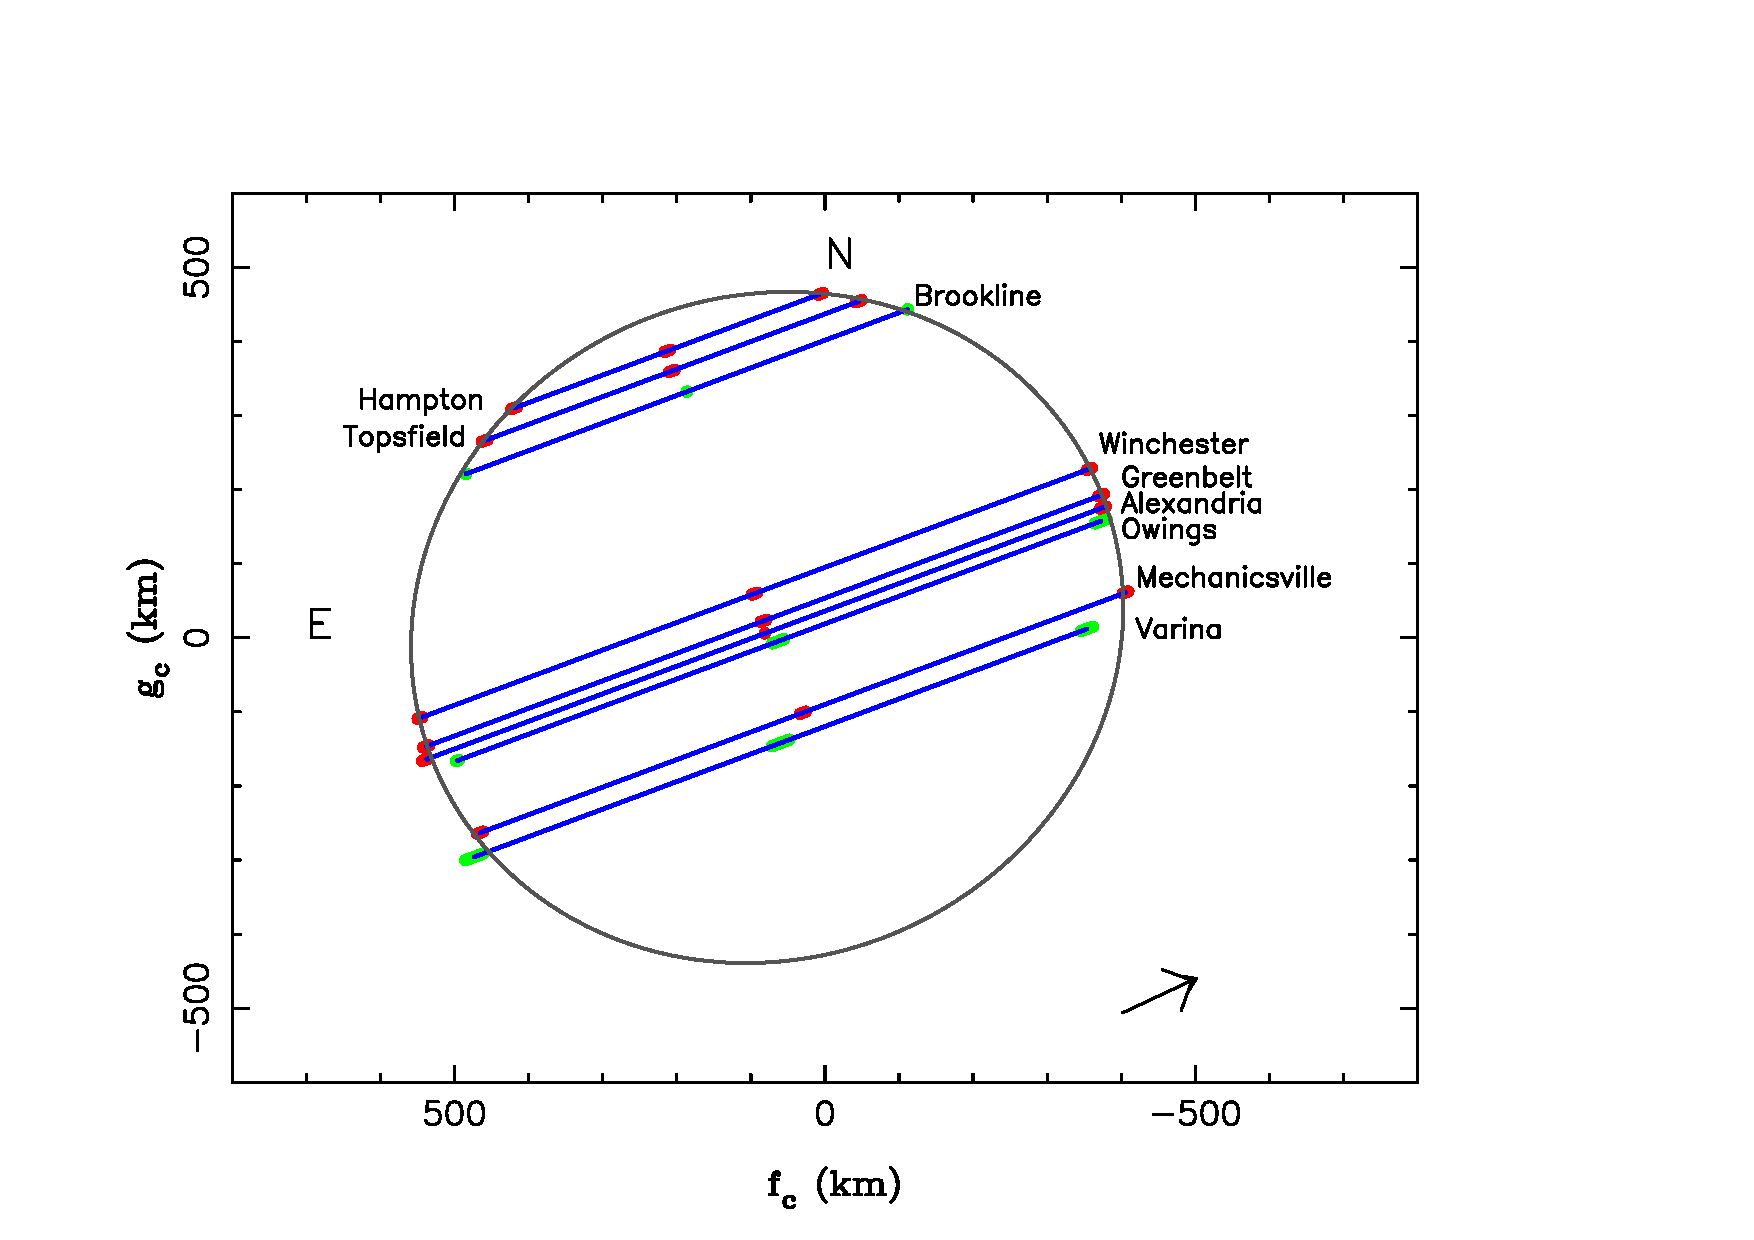
\includegraphics[scale=0.36]{figures/Ceres_2013_body.pdf}
\caption{\label{Fig: Ceres-2013-body}}
\end{figure}

\section[]{Discussion}






\section{Conclusions}



\section*{Acknowledgments}

Agradecimentos


\begin{thebibliography}{99}

\bibitem[\protect\citeauthoryear{Assafin et al}{2011}] {2011gfun.conf...85A} Assafin M. et al., 2011, Gaia follow-up network for the solar system objects : Gaia FUN-SSO workshop proceedings, held at IMCCE -Paris Observatory, France, November 29 - December 1, 2010. ISBN 2-910015-63-7

%@INPROCEEDINGS{2011gfun.conf...85A,
%   author = {{Assafin}, M. and {Vieira Martins}, R. and {Camargo}, J.~I.~B. and 
%	{Andrei}, A.~H. and {Da Silva Neto}, D.~N. and {Braga-Ribas}, F.
%	},
%    title = "{PRAIA - Platform for Reduction of Astronomical Images Automatically}",
%booktitle = {Gaia follow-up network for the solar system objects : Gaia FUN-SSO workshop proceedings, held at IMCCE -Paris Observatory, France, November 29 - December 1, 2010. ISBN 2-910015-63-7},
%     year = 2011,
%   editor = {{Tanga}, P. and {Thuillot}, W.},
%    month = jun,
%    pages = {85-88},
%   adsurl = {http://adsabs.harvard.edu/abs/2011gfun.conf...85A},
%  adsnote = {Provided by the SAO/NASA Astrophysics Data System}
%}

\bibitem[\protect\citeauthoryear{Braga-Ribas et al.}{2013}]{BragaRibas2013} Braga-Ribas F. et al., 2013,
ApJ, 773, 26

\bibitem[\protect\citeauthoryear{Braga-Ribas et al.}{2014}]{BragaRibas2014} Braga-Ribas F. et al., 2014,
Nature, 508, 72

\bibitem[\protect\citeauthoryear{Drummond et al.}{2014}]{Drummond2014} Drummond J.D. et al., 2014,
Icarus, 236, 28

\bibitem[\protect\citeauthoryear{Hog E. et al}{2000}] {Hog2000} Hog E. et al. 2000, A\&A, 355, L27-30 (2000)

\bibitem[\protect\citeauthoryear{K\"{u}ppers et al.}{2014}]{Kuppers2014} K\"{u}ppers M. et al., 2014,
Nature, 505, 525

\bibitem[\protect\citeauthoryear{Millis et al.}{1987}]{Millis1987} Millis R.L. et al., 1987,
Icarus, 72, 507

\bibitem[\protect\citeauthoryear{Ortiz et al.}{2012}]{Ortiz2012} Ortiz J. L. et al., 2012,
Nature, 491, 566

\bibitem[\protect\citeauthoryear{Sicardy et al.}{2011}]{Sicardy2011} Sicardy B. et al., 2011,
Nature, 478, 493

\bibitem[\protect\citeauthoryear{Widemann et al.}{2009}] {Widemann2009} Widemann, T., Sicardy, B., Dusser, R., et al. 2009, Icarus, 199, 458

\bibitem[\protect\citeauthoryear{van Belle}{1999}] {vanBelle1999} van Belle, G. T. 1999, PASP, 111, 1515


















%Artigos do exemplo

%\bibitem[\protect\citeauthoryear{Dawson}{1979}]{b4} Dawson D.W., 1979,
%ApJS, 41, 97
%\bibitem[\protect\citeauthoryear{Gerhz}{1972}]{b5} Gerhz R.D., 1972, ApJ,
%178, 715
%\bibitem[\protect\citeauthoryear{Gerhz \& Ney}{1972}]{b6} Gerhz R.D., Ney
%E.P., 1972, PASP, 84, 768
%\bibitem[\protect\citeauthoryear{Gerhz \& Woolf}{1970}]{b7} Gerhz R.D., Woolf N.J.,
%1970, ApJ, 161, L213
%\bibitem[\protect\citeauthoryear{Gilman}{1972}]{b8} Gilman R.C., 1972, ApJ, 178, 423
%\bibitem[\protect\citeauthoryear{Goldsmith et al.}{1987}]{b9} Goldsmith M.J., Evans A.,
%Albinson J.S., Bode M.F., 1987, MNRAS, 227, 143
%\bibitem[\protect\citeauthoryear{Hacking et al.}{1985}]{b10} Hacking P. et al., 1985,
%PASP, 97, 616
%\bibitem[\protect\citeauthoryear{Harvey, Thronson \& Gatley}{Harvey et al.}{1979}]{b11}
%Harvey P.M., Thronson H.A., Gatley I., 1979, ApJ, 231, 115
%\bibitem[\protect\citeauthoryear{Jura}{1986}]{b12} Jura M., 1986, ApJ, 309, 732
%\bibitem[\protect\citeauthoryear{Kukarkin et al.}{1969}]{b13} Kukarkin B.V. et al.,
%1969, General Catalogue of Variable Stars. Moscow
%\bibitem[\protect\citeauthoryear{Lloyd Evans}{1974}]{b14} Lloyd Evans T., 1974, MNRAS,
%167, 17{\sc p}
%\bibitem[\protect\citeauthoryear{Lloyd Evans}{1985}]{b15} Lloyd Evans T., 1985, MNRAS,
%217, 493
%\bibitem[\protect\citeauthoryear{Low et al.}{1984}]{b16} Low F.J. et al., 1984, ApJ,
%278, L19
%\bibitem[\protect\citeauthoryear{McLaughlin}{1932}]{b17} McLaughlin D.B., 1932, Publ. Univ.
%Obs. Mich., 4, 135
%\bibitem[\protect\citeauthoryear{O'Connell}{1961}]{b18} O'Connell J.K., 1961, Specola
%Vaticana Ric. Astron., 6, 341
%\bibitem[\protect\citeauthoryear{Olnon \& Raimond}{1986}]{b19} Olnon F.M., Raimond E., 1986,
%A\&AS, 65, 607
%\bibitem[\protect\citeauthoryear{Preston et al.}{1963}]{b20} Preston G.W., Krzeminski W., Smak J.,
%Williams J.A., 1963, ApJ, 137, 401
%\bibitem[\protect\citeauthoryear{Rowan-Robinson \& Harris}{1983a}]{b21} Rowan-Robinson M., Harris
%S., 1983a, MNRAS, 202, 767
%\bibitem[\protect\citeauthoryear{Rowan-Robinson \& Harris}{1983b}]{b22} Rowan-Robinson M., Harris
%S., 1983b, MNRAS, 202, 797
%\bibitem[\protect\citeauthoryear{van der Veen \& Habing}{1988}]{b23} van der Veen W.E.C.J., Habing
%H.J., 1988, A\&A, 194, 125
%\bibitem[\protect\citeauthoryear{Willems \& de Jong}{1988}]{b24} Willems F.J., de Jong T., 1988,
%A\&A, 196, 173
%\bibitem[\protect\citeauthoryear{Zuckerman \& Dyck}{1986}]{b25} Zuckerman B., Dyck H.M., 1986, ApJ,
%311, 345
\end{thebibliography}



%\bsp

\label{lastpage}

\end{document}